\subsubsection{Kernel, Identity Mapping}
Debemos mapear con Identity mapping las direcciones 0x00000000 a 0x00DC3FFF. Para esto fueron necesarios:
\begin{itemize}
 \item 1 Tabla de Directorios de p\'aginas que empieza en la direccion 0x27000.
 \item 4 Entradas de tabla de directorios. 
 \item 4 tablas de p\'aginas. La 3 primeras Page table posee sus 1024 entradas completas  
y tienen como base la direcci\'on 0x28000, 0x30000,0x32000 respectivamente. Y la cuarta tabla con 452 entradas presentes. \\
De esta forma conseguimos mapear todas las direcciones
\end{itemize}

Las entradas de directorio para Kernel son cargadas de la siguiente manera\footnote{Se pueden considerar a los flags no declarados como
no seteados, es decir, iguales a 0.}:
\begin{itemize}
 \item P = 1.
 \item R/W = 1.
 \item U/S = 0.
 \item Direccion de la Page Table = 0x28000,0x30000,0x32000 seg\'un corresponda la  page table.
\end{itemize}

Las entradas de Page Table para el Kernel son cargadas de la siguiente manera\footnotemark[3]:
\begin{itemize}
 \item P = 1.
 \item R/W = 1.
 \item U/S = 0.
 \item Direccion del Page Frame desde 0x00000000 a 0x00DC3FFF seg\'un corresponda.
\end{itemize}

A continuaci\'on se detalla un esquema para una mejor comprensi\'on de lo explicado:

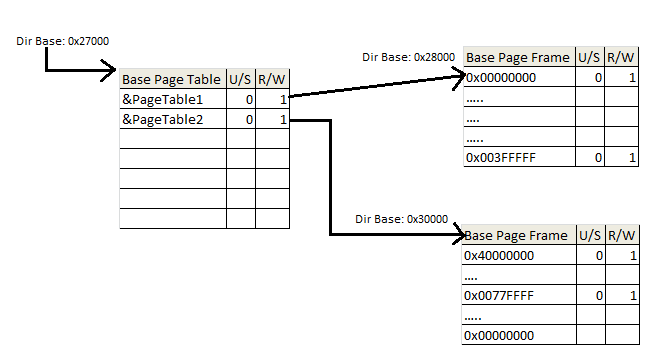
\includegraphics[scale=0.6]{imagenes/tablasDePaginasEj3.png}

\subsubsection{Activaci\'on de paginaci\'on}

Luego de armar el directorio de p\'aginas podemos habilitar la paginaci\'on. Para esto seguimo los siguientes pasos:
\begin{itemize}
 \item Cargar en CR3 la direccion al inicio del directorio de p\'aginas.
 \item Setear el bit mas significativo del registro CR0.
\end{itemize}

